\documentclass[conference]{IEEEtran}
\IEEEoverridecommandlockouts
% Times/Courier clones when compiled with XeTeX (e.g. Tectonic); pdfLaTeX/Overleaf skip this
\usepackage{iftex}
\ifXeTeX
  \usepackage{fontspec}
  \setmainfont{texgyretermes}[Extension=.otf, UprightFont=*-regular,
    BoldFont=*-bold, ItalicFont=*-italic, BoldItalicFont=*-bolditalic]
  \setmonofont{texgyrecursor}[Extension=.otf, UprightFont=*-regular,
    BoldFont=*-bold, ItalicFont=*-italic, BoldItalicFont=*-bolditalic]
\fi
\usepackage{cite}
\usepackage{amsmath,amssymb,amsfonts}
\usepackage{graphicx}
\usepackage{textcomp}
\usepackage{xcolor}
\usepackage{booktabs}
\usepackage{listings}
\usepackage{tikz}
\usetikzlibrary{positioning,arrows.meta}
\usepackage{url}

\lstset{
  language=Python,
  basicstyle=\ttfamily\scriptsize,
  keywordstyle=\color{blue!60!black},
  commentstyle=\color{gray},
  stringstyle=\color{green!40!black},
  columns=fullflexible,
  keepspaces=true,
  upquote=true,
  frame=tb,
  aboveskip=4pt,
  belowskip=2pt,
  xleftmargin=2pt,
  captionpos=b
}

\begin{document}

\title{Griev.AI.ance: Routing Consumer Financial Complaints with Machine Learning\\
{\large CSC 4850 Mid-Project Report}}

\author{
\IEEEauthorblockN{Raina Bethea}
\IEEEauthorblockA{\textit{Dept. of Computer Science}\\
\textit{Georgia State University}\\
Atlanta, GA, USA}
\and
\IEEEauthorblockN{Omar Elkady}
\IEEEauthorblockA{\textit{Dept. of Computer Science}\\
\textit{Georgia State University}\\
Atlanta, GA, USA}
\and
\IEEEauthorblockN{Victor Googe}
\IEEEauthorblockA{\textit{Dept. of Computer Science}\\
\textit{Georgia State University}\\
Atlanta, GA, USA}
}

\maketitle

\begin{abstract}
Griev.AI.ance (repository: ComplaintRouter) reads the free-text narrative of a complaint filed with the U.S.\ Consumer Financial Protection Bureau (CFPB) and predicts its financial product among 11 categories; a secondary goal is to predict whether the complaint will close with monetary relief. So far we have cleaned 2.32 million narratives filed between September 2023 and August 2026, drawn a 162,500-complaint sample with per-product caps, completed an exploratory analysis, and trained a TF-IDF + multinomial naive Bayes baseline that reaches 72.9\% accuracy and 0.69 macro-F1 on a held-out test set. We describe the data, the baseline and its failure modes, and our week-by-week plan for the remaining work.
\end{abstract}

\begin{IEEEkeywords}
text classification, consumer complaints, CFPB, TF-IDF, naive Bayes
\end{IEEEkeywords}

\section{Introduction}
The CFPB forwards complaints about credit reports, debt collectors, bank accounts, loans and other consumer financial products to the companies involved and publishes them in its Consumer Complaint Database~\cite{cfpb}. A single two-month export (March--April 2025) holds 803,073 complaints. Each complaint carries the product the consumer selected when filing and must reach the team that handles that product; misrouting slows resolution, and complaints likely to end in monetary relief deserve priority. A model that reads the narrative can route new complaints, flag labels that look inconsistent with the text, and support triage.

We frame routing as supervised multi-class text classification: the input is the consumer's narrative and the target is one of 11 CFPB product categories. We represent narratives with TF-IDF features and compare classical classifiers under one protocol, with macro-F1 as the primary metric because the classes are imbalanced. Our goals are (1)~an accurate, interpretable product classifier; (2)~a binary model for the rare monetary-relief outcome; (3)~an analysis of the text's structure with truncated SVD and $k$-means clustering; and (4)~a small interactive demo. At the midpoint, the data pipeline, the exploratory analysis and a naive Bayes baseline are complete (Fig.~\ref{fig:map}).

\section{Related Work}
\textit{Classical text categorization.} Joachims~\cite{joachims} showed that linear SVMs suit text, with its many sparse but relevant features, and outperformed naive Bayes, Rocchio, $k$-NN and C4.5 on the Reuters and Ohsumed benchmarks. McCallum and Nigam~\cite{mccallum} found that the multinomial event model of naive Bayes beats the multivariate Bernoulli model, especially with large vocabularies, and Rennie et al.~\cite{rennie} corrected several naive Bayes assumptions (for example with Complement NB), closing much of the gap to SVMs on skewed class distributions. Latent semantic analysis~\cite{lsa} applies a truncated SVD to the term--document matrix to obtain dense, low-rank text representations. These results motivate our progression from naive Bayes to linear models and our use of truncated SVD.

\textit{CFPB complaints.} Bastani et al.~\cite{bastani} built a decision-support system that applies LDA topic modeling to CFPB narratives to surface consumer issues automatically and to examine the effect of federal consumer-protection regulations. Pradhan et al.~\cite{pradhan} classify CFPB complaints with large language models: supplying the most similar labeled complaints as few-shot examples consistently beat zero-shot prompting and also outperformed fine-tuned RoBERTa, SVM and logistic-regression baselines.

\textit{Monetary relief.} Wang et al.~\cite{wang} predict whether a complaint closes with monetary relief as an imbalanced binary problem. Their XGBoost model combines narrative text, LDA topics, engineered text features and company/state fields, is evaluated on a temporal split, and raises ROC-AUC from 0.69 (a TF-IDF baseline) to 0.78. In our project, product routing is the primary task, all classical models share one split, and relief prediction is secondary, with~\cite{wang} as a reference point.

\begin{figure*}[!t]
\centering
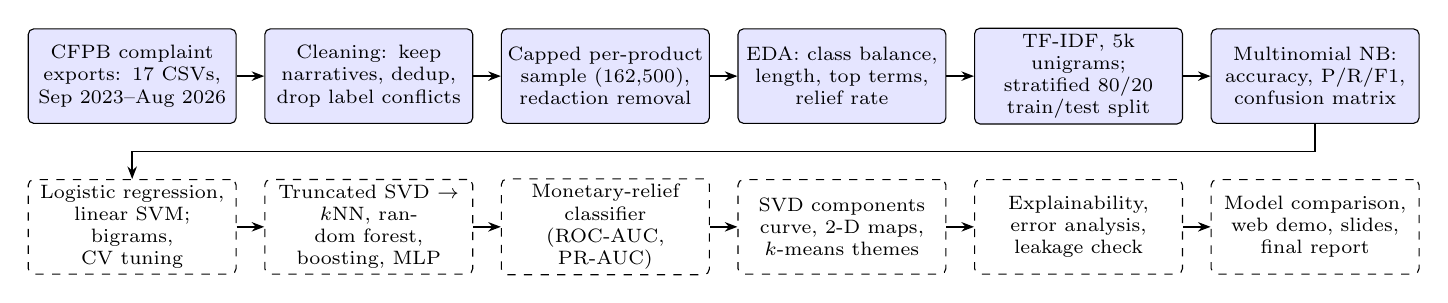
\begin{tikzpicture}[
  node distance=3mm and 3.5mm,
  stage/.style={draw, rounded corners=2pt, align=center, font=\scriptsize,
                text width=25mm, minimum height=12mm, inner sep=2pt},
  done/.style={stage, fill=blue!10},
  todo/.style={stage, dashed},
  arr/.style={-{Stealth[length=1.6mm]}, semithick}]
\node[done] (data) {CFPB complaint\\exports: 17 CSVs,\\Sep 2023--Aug 2026};
\node[done, right=of data] (clean) {Cleaning: keep\\narratives, dedup,\\drop label conflicts};
\node[done, right=of clean] (sample) {Capped per-product\\sample (162,500),\\redaction removal};
\node[done, right=of sample] (eda) {EDA: class balance,\\length, top terms,\\relief rate};
\node[done, right=of eda] (tfidf) {TF-IDF, 5k unigrams;\\stratified 80/20\\train/test split};
\node[done, right=of tfidf] (nb) {Multinomial NB:\\accuracy, P/R/F1,\\confusion matrix};
\node[todo, below=7mm of data] (lin) {Logistic regression,\\linear SVM; bigrams,\\CV tuning};
\node[todo, right=of lin] (nonlin) {Truncated SVD $\rightarrow$\\$k$NN, random forest,\\boosting, MLP};
\node[todo, right=of nonlin] (relief) {Monetary-relief\\classifier\\(ROC-AUC, PR-AUC)};
\node[todo, right=of relief] (clus) {SVD components\\curve, 2-D maps,\\$k$-means themes};
\node[todo, right=of clus] (expl) {Explainability,\\error analysis,\\leakage check};
\node[todo, right=of expl] (demo) {Model comparison,\\web demo, slides,\\final report};
\foreach \a/\b in {data/clean, clean/sample, sample/eda, eda/tfidf, tfidf/nb,
                   lin/nonlin, nonlin/relief, relief/clus, clus/expl, expl/demo}
  \draw[arr] (\a) -- (\b);
\draw[arr] (nb.south) -- ++(0,-3.5mm) -| (lin.north);
\end{tikzpicture}
\caption{Project map. Shaded boxes (top row) are complete; dashed boxes (bottom row) are the remaining work, in the order scheduled in Table~\ref{tab:plan}.}
\label{fig:map}
\end{figure*}

\section{Methodology}
Fig.~\ref{fig:map} maps the project. Narratives are cleaned, sampled and converted into TF-IDF vectors $\mathbf{x}\in\mathbb{R}^{|V|}$. Our first classifier is multinomial naive Bayes (MNB), which predicts
\begin{equation}
\hat{c} = \arg\max_{c}\Big[\log \pi_c + \sum_{j} x_j \log \theta_{cj}\Big],\quad
\theta_{cj} = \frac{N_{cj}+\alpha}{N_c+\alpha|V|},
\end{equation}
where $\pi_c$ is the class prior, $N_{cj}$ is the total weight of term $j$ in class $c$, and $\alpha$ is the smoothing constant. MNB trains in a single pass and is a standard text baseline~\cite{mccallum}.

Next we will train logistic regression and a linear SVM directly on the sparse TF-IDF matrix, and $k$-nearest neighbors, random forest, gradient boosting and a multilayer perceptron on a truncated-SVD projection, since trees and neighbor search scale poorly to thousands of sparse dimensions. Truncated SVD also supports 2-D visualization and $k$-means clustering of complaint themes. The relief task will reuse these features with class-weighted linear models. Hyperparameters will be tuned with stratified cross-validation on the training set only. Routing is scored with accuracy, per-class precision, recall and F1, and macro-F1; relief, whose positives are rare, with ROC-AUC and PR-AUC.

\section{Dataset Description}
\label{sec:data}
\textit{Source.} We use the CFPB Consumer Complaint Database~\cite{cfpb}. Each record has 16 fields, including the product, issue, company, company response and narrative. Narratives are published only with the consumer's consent, after personal information is replaced with placeholders such as \texttt{XXXX}. We downloaded 17 CSV exports covering complaints received from September 1, 2023 to August 11, 2026, all after the CFPB's August 2023 revision of its product categories, so the 11 product labels are consistent. Only about a quarter of complaints include a narrative (26.2\% in the March--April 2025 export).

\textit{Pre-processing.} Table~\ref{tab:funnel} summarizes the cleaning steps. We kept 10 relevant columns and dropped complaints without a narrative, leaving 2,323,440. Exact duplicates are common: 1,007,818 narratives (43.4\%) repeat an earlier one, mostly mass-produced dispute letters (the most repeated text, a Fair Credit Reporting Act template, appears 26,154 times). We removed the 1,650 narratives filed under more than one product, whose label is ambiguous, and kept one copy of each remaining narrative. Because credit reporting makes up 57\% of the de-duplicated data, we drew a random sample capped per product (35,000 for credit reporting down to 5,000 for prepaid cards and debt or credit management; seed 42), giving 162,500 complaints. Finally, we lowercased the text, removed redaction placeholders (\texttt{XX}, \texttt{XXXX}) and runs of zeros, and collapsed whitespace; six narratives that became empty were dropped, leaving 162,494.

\begin{table}[!t]
\caption{Data cleaning funnel}
\label{tab:funnel}
\centering
\footnotesize
\begin{tabular}{@{}lr@{}}
\toprule
Stage & Narratives \\
\midrule
With a narrative (17 exports) & 2,323,440 \\
After removing exact duplicates & 1,315,622 \\
After removing conflicting product labels & 1,313,972 \\
Capped per-product sample & 162,500 \\
Non-empty after text cleaning & 162,494 \\
\bottomrule
\end{tabular}
\end{table}

\section{Exploratory Data Analysis}
\textit{Missing values and duplicates.} After de-duplication only two fields have missing values: sub-issue (92,687 rows, 7.0\%) and company response (3 rows); narrative and product are always present. Template letters (Section~\ref{sec:data}) were the main data-quality problem.

\textit{Class balance.} In the de-duplicated data the largest product (credit reporting, 752,276 narratives) is 137 times larger than the smallest (debt or credit management, 5,482). The capped sample reduces this ratio to 7:1 (Fig.~\ref{fig:classes}) while keeping every class large enough to learn.

\begin{figure}[!t]
\centering
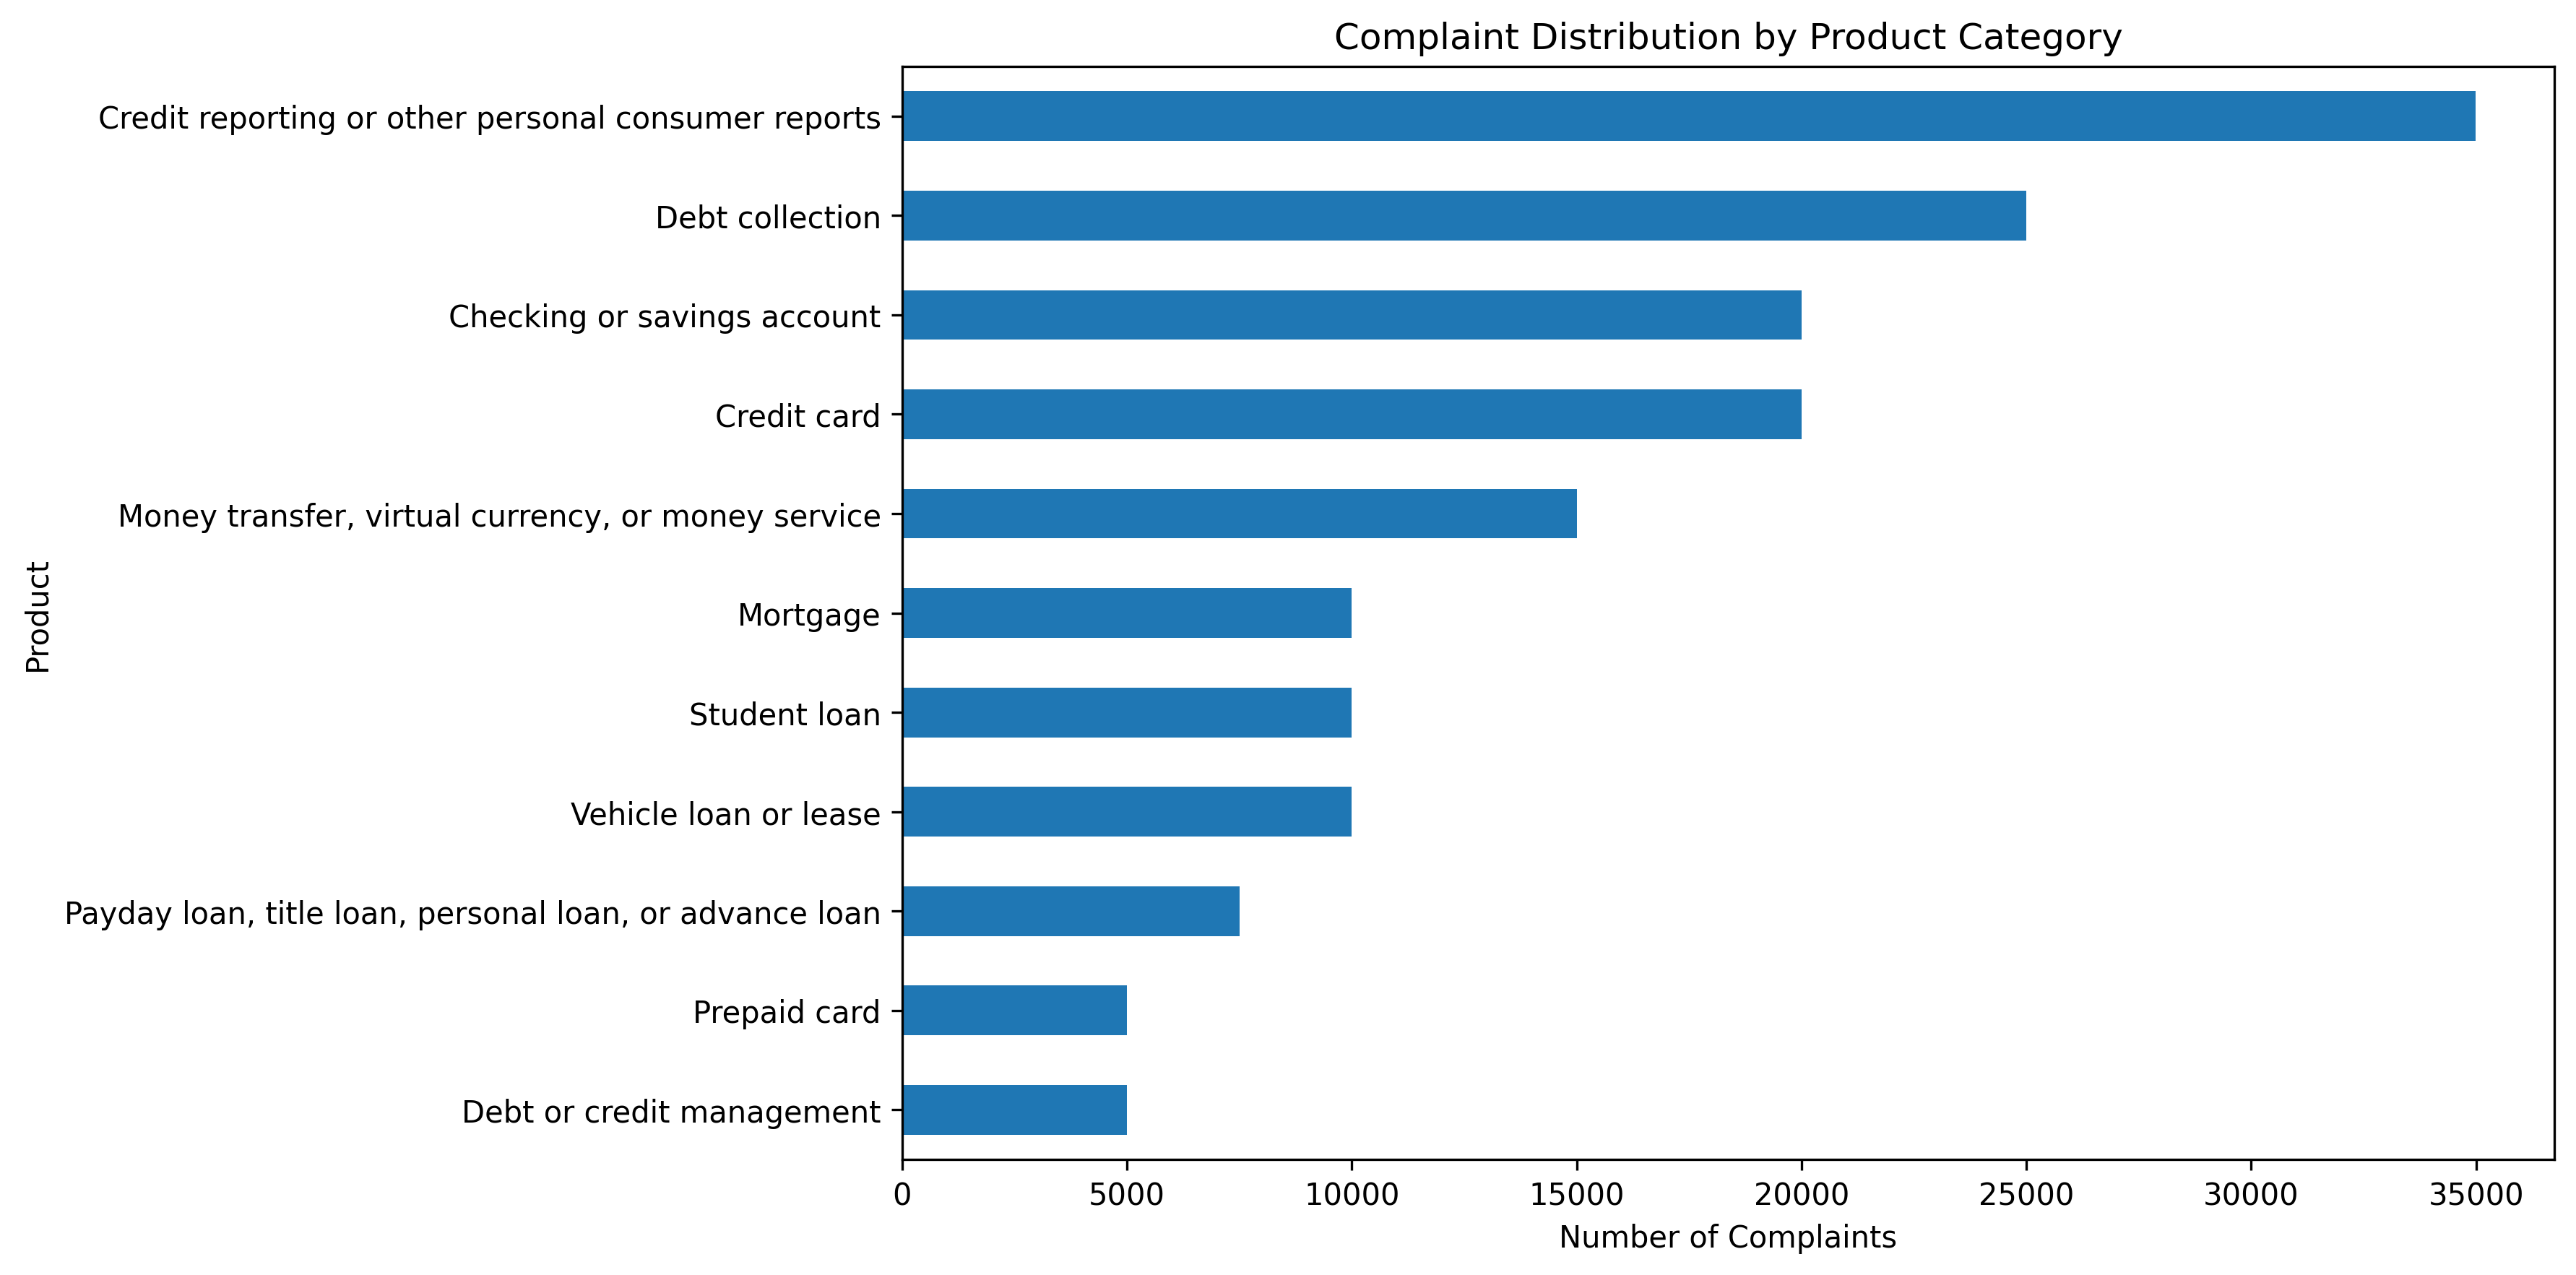
\includegraphics[width=0.9\columnwidth]{figures/product_class_distribution.png}
\caption{Complaints per product in the 162,500-complaint modeling sample.}
\label{fig:classes}
\end{figure}

\textit{Narrative length.} Lengths are right-skewed (Fig.~\ref{fig:length}): the median is 157 words, the mean 217, the interquartile range 83--273 and the maximum 5,911. Mortgage narratives are the longest (median 221 words) and money-transfer narratives the shortest (median 108). We keep the long tail, since TF-IDF vectors are L2-normalized.

\begin{figure}[!t]
\centering
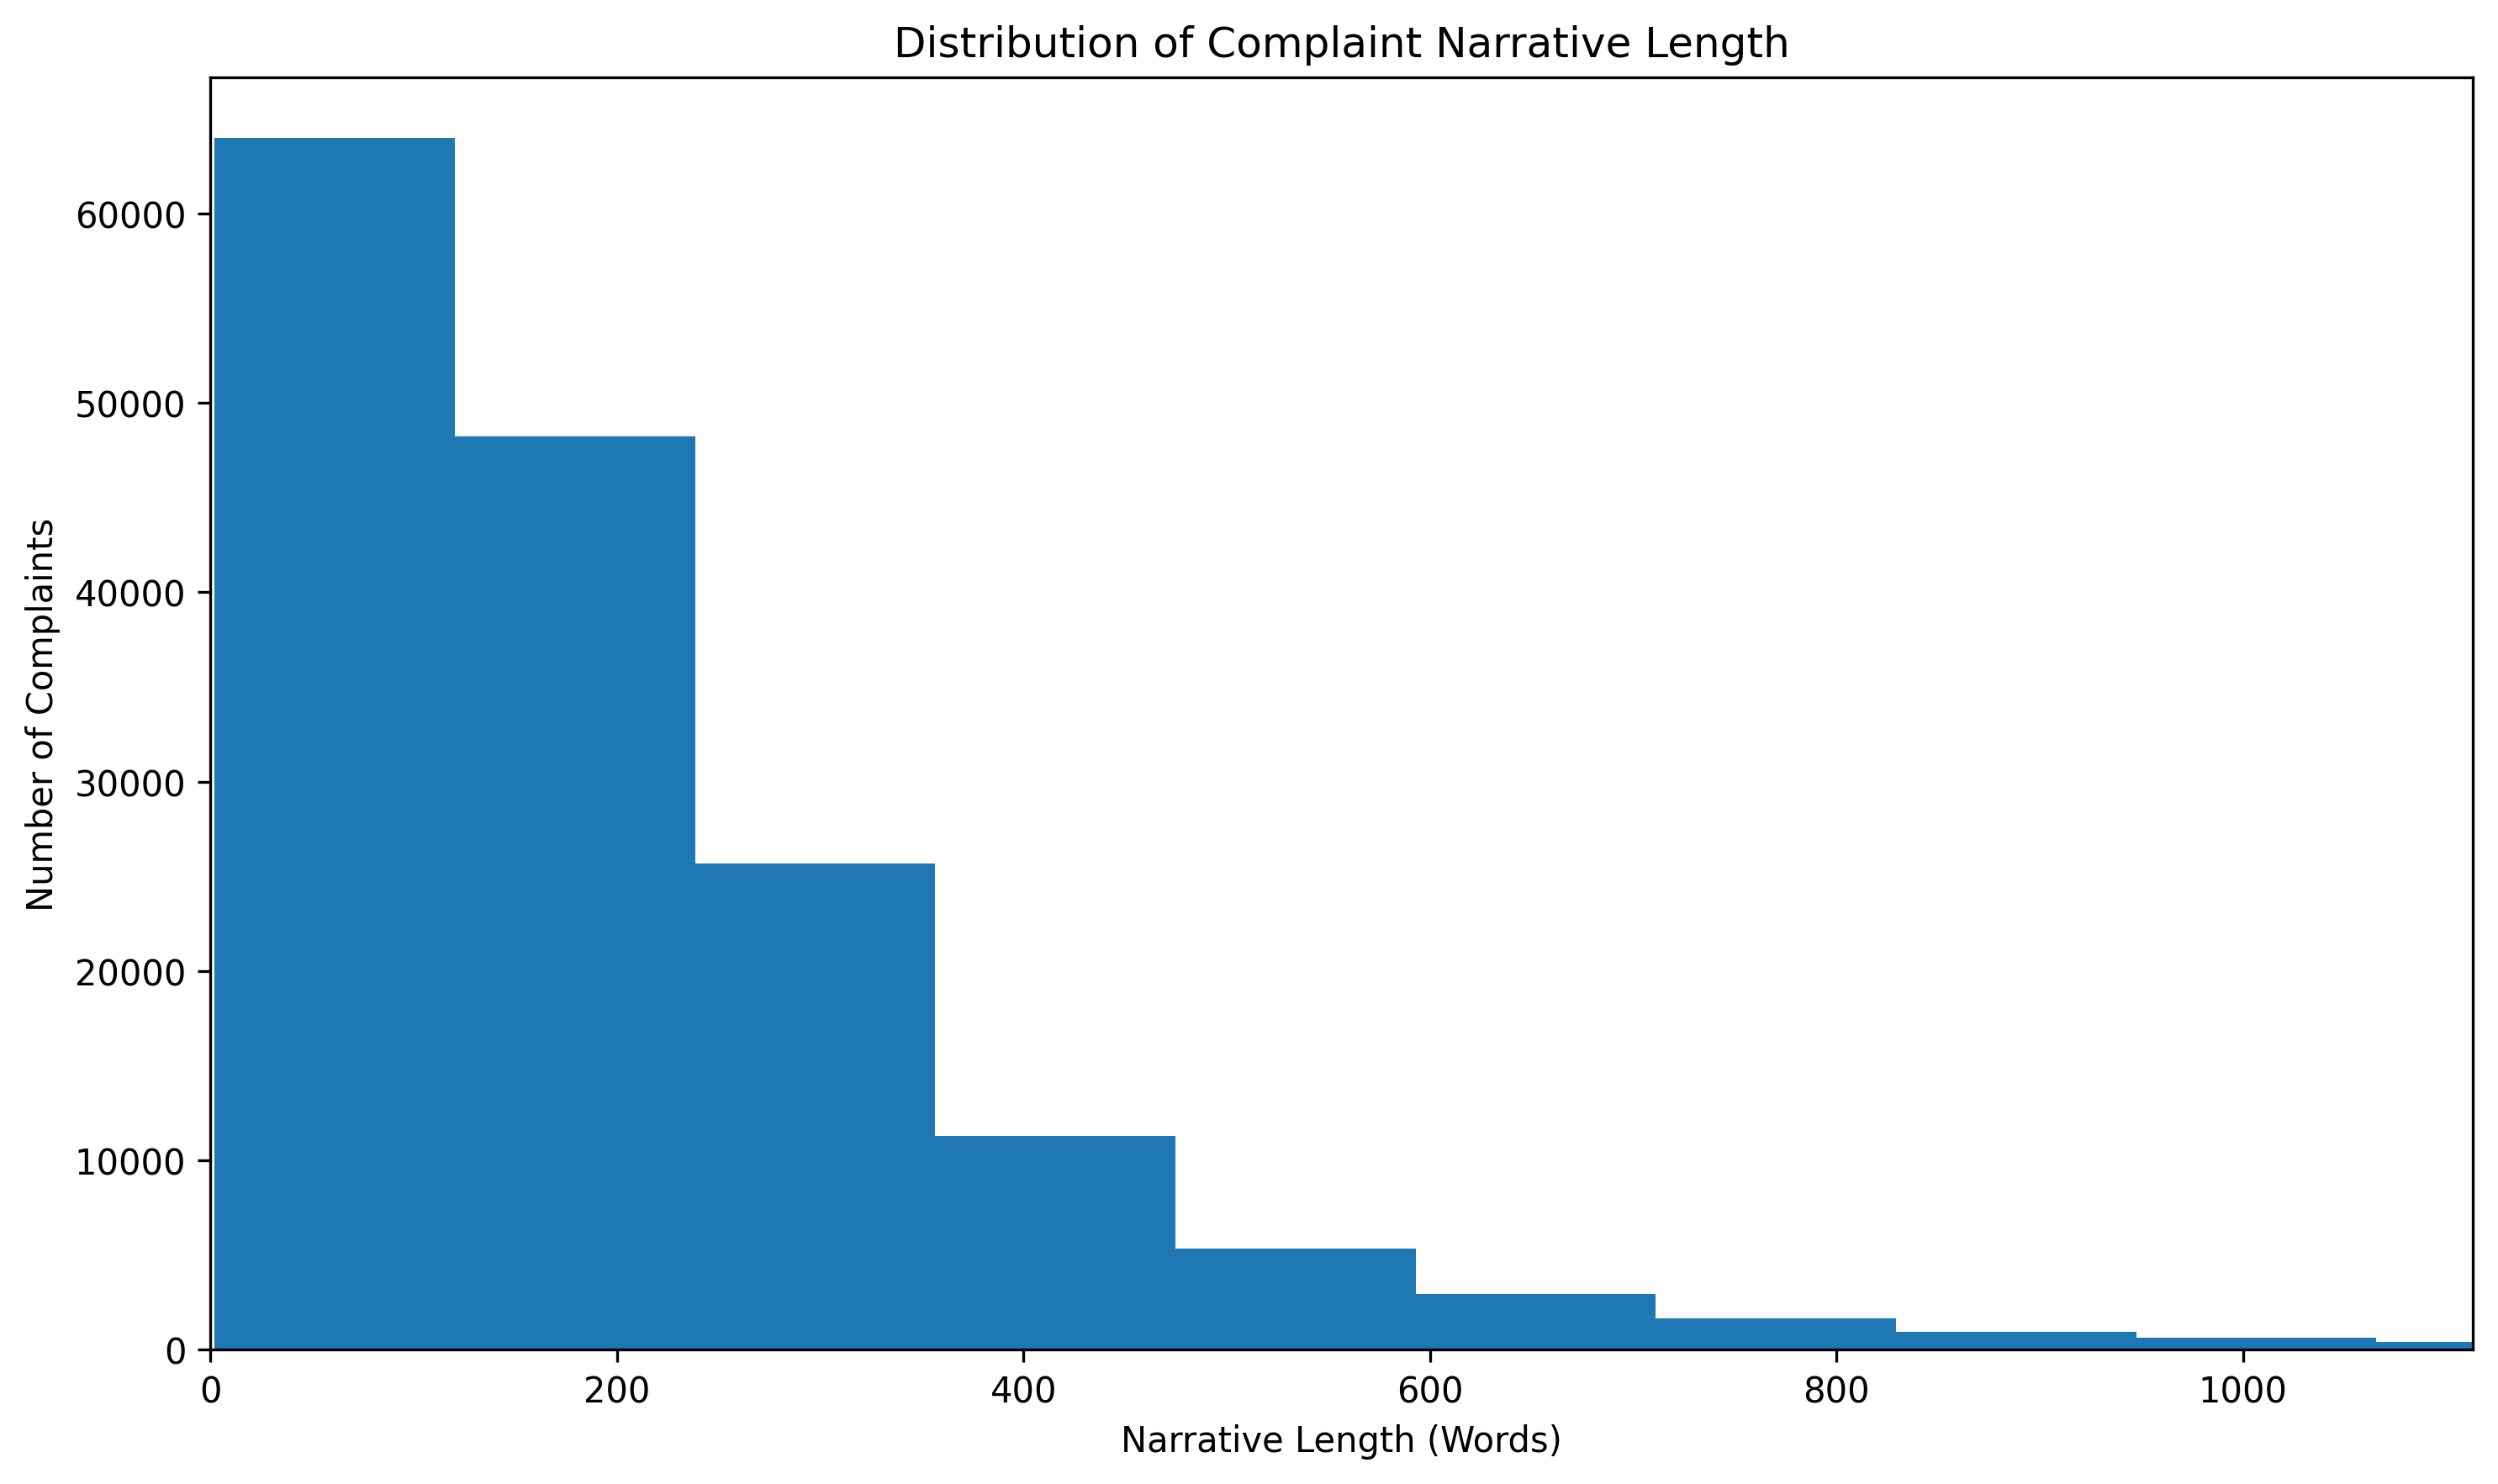
\includegraphics[width=0.7\columnwidth]{figures/narrative_length_distribution.png}
\caption{Narrative length in words (x-axis clipped at the 99th percentile).}
\label{fig:length}
\end{figure}

\textit{Vocabulary.} Table~\ref{tab:terms} lists the terms with the highest mean TF-IDF weight in each product. The top-ten lists show distinctive vocabulary for several classes, including company names (\textit{mohela} and \textit{nelnet} for student loans, \textit{zelle}, \textit{cash} and \textit{app} for money transfer, \textit{amex} for prepaid cards), legal terms (\textit{fcra} for credit reporting) and product terms (\textit{escrow}, \textit{foreclosure}). Other classes share generic words such as \textit{credit}, \textit{account}, \textit{debt} and \textit{payment}, which foreshadows the confusions in Section~\ref{sec:exp}. Before cleaning, the placeholder \texttt{XXXX} ranked among the top terms of nearly every class, which is why we removed it.

\begin{table}[!t]
\caption{Top five TF-IDF terms per product (modeling sample)}
\label{tab:terms}
\centering
\scriptsize
\begin{tabular}{@{}p{0.27\columnwidth}p{0.67\columnwidth}@{}}
\toprule
Product & Top terms \\
\midrule
Credit reporting & credit, report, information, reporting, consumer \\
Debt collection & debt, credit, collection, account, report \\
Credit card & card, credit, account, bank, payment \\
Checking/savings & account, bank, funds, money, check \\
Money transfer & app, cash, account, zelle, money \\
Mortgage & mortgage, loan, payment, escrow, insurance \\
Student loan & loans, loan, mohela, student, payment \\
Vehicle loan/lease & vehicle, car, loan, payment, credit \\
Payday/personal loan & loan, payment, account, payments, pay \\
Prepaid card & card, gift, use, cards, money \\
Debt/credit mgmt. & credit, debt, account, company, report \\
\bottomrule
\end{tabular}
\end{table}

\textit{Outcomes.} Most complaints close with an explanation (77.0\%); 16.1\% end in non-monetary relief, 5.6\% in monetary relief, 1.2\% receive an untimely response, and 37 are still in progress. Relief of either kind is most common for credit reporting (43.3\%, typically corrections) and credit cards (30.1\%) and rarest for student loans (2.4\%) (Fig.~\ref{fig:relief}). Because monetary relief occurs in only 5.6\% of complaints, the planned relief model needs imbalance-aware metrics such as PR-AUC.

\begin{figure}[!t]
\centering
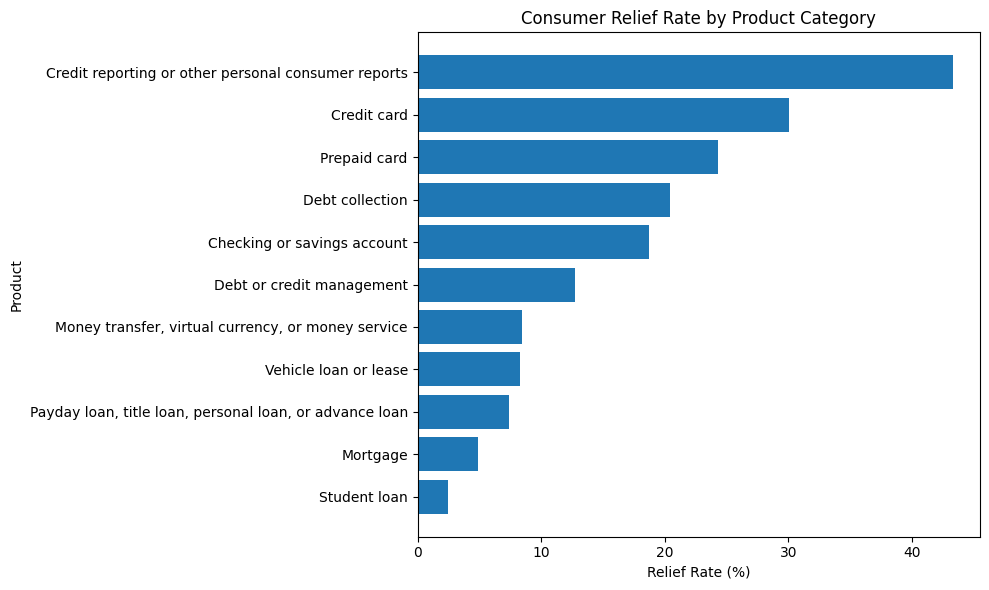
\includegraphics[width=0.85\columnwidth]{figures/relief_rate_by_product.png}
\caption{Share of complaints closed with monetary or non-monetary relief, by product.}
\label{fig:relief}
\end{figure}

\section{Experiments}
\label{sec:exp}
\textit{Setup.} We split the 162,494 complaints 80/20 with stratification by product (129,995 training and 32,499 test complaints; seed 42). The TF-IDF vectorizer removes English stop words, keeps unigrams that appear in at least five documents, and retains the 5,000 most frequent terms; it is fitted on the training set only, so no test vocabulary leaks into training. MNB uses the scikit-learn~\cite{sklearn} defaults ($\alpha=1$, class priors estimated from the training data). Listing~\ref{lst:nb} shows the core of the experiment.

\begin{lstlisting}[float=!t, caption={Text cleaning and the naive Bayes baseline (abridged).}, label=lst:nb]
def clean_narrative(text):
    text = str(text).lower()
    text = re.sub(r'\bx{2,}\b', ' ', text)  # redactions
    text = re.sub(r'\b0{2,}\b', ' ', text)  # zero runs
    return re.sub(r'\s+', ' ', text).strip()
X_train, X_test, y_train, y_test = train_test_split(
    df["clean_narrative"], df["Product"], test_size=0.20,
    random_state=42, stratify=df["Product"])
vectorizer = TfidfVectorizer(stop_words="english",
                             max_features=5000, min_df=5)
X_train_tfidf = vectorizer.fit_transform(X_train)
X_test_tfidf = vectorizer.transform(X_test)  # no refit
nb_model = MultinomialNB().fit(X_train_tfidf, y_train)
y_pred = nb_model.predict(X_test_tfidf)
\end{lstlisting}

\textit{Results.} On the test set MNB reaches 72.9\% accuracy and 0.69 macro-F1 (macro precision 0.78, macro recall 0.67; weighted F1 0.72). Table~\ref{tab:nb} gives per-class scores and Fig.~\ref{fig:cm} the confusion matrix.

\begin{table}[!t]
\caption{Naive Bayes test results per product}
\label{tab:nb}
\centering
\footnotesize
\begin{tabular}{@{}lrrrr@{}}
\toprule
Product & Precision & Recall & F1 & Support \\
\midrule
Checking/savings & 0.57 & 0.86 & 0.68 & 4,000 \\
Credit card & 0.63 & 0.73 & 0.68 & 4,000 \\
Credit reporting & 0.76 & 0.85 & 0.80 & 6,999 \\
Debt collection & 0.74 & 0.68 & 0.71 & 5,000 \\
Debt/credit mgmt. & 0.79 & 0.25 & 0.38 & 1,000 \\
Money transfer & 0.90 & 0.53 & 0.67 & 3,000 \\
Mortgage & 0.87 & 0.88 & 0.87 & 2,000 \\
Payday/personal loan & 0.72 & 0.45 & 0.56 & 1,500 \\
Prepaid card & 0.87 & 0.51 & 0.64 & 1,000 \\
Student loan & 0.90 & 0.86 & 0.88 & 2,000 \\
Vehicle loan/lease & 0.80 & 0.72 & 0.76 & 2,000 \\
\midrule
Macro average & 0.78 & 0.67 & 0.69 & 32,499 \\
\bottomrule
\end{tabular}
\end{table}

\begin{figure}[!t]
\centering
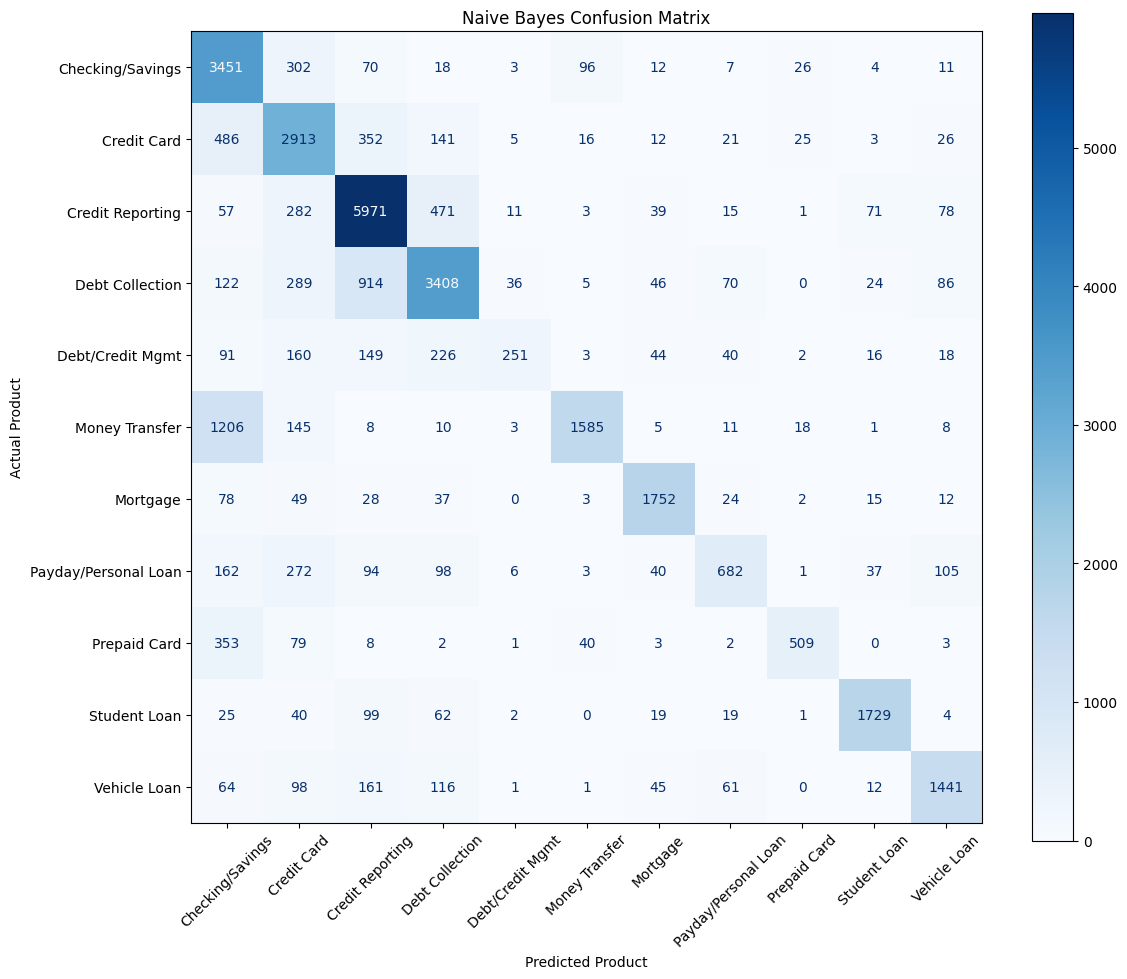
\includegraphics[width=0.88\columnwidth]{figures/naive_bayes_confusion_matrix.png}
\caption{Naive Bayes confusion matrix on the 32,499-complaint test set (rows: actual product; columns: predicted product).}
\label{fig:cm}
\end{figure}

\textit{Training and validation loss.} MNB has no iterative optimization: its parameters in (1) are smoothed relative frequencies computed in one pass over the training data, so this experiment has no per-epoch loss curve. Next we will plot training and validation log-loss against training-set size for naive Bayes and logistic regression, and per-epoch training and validation loss for the MLP, which holds out a validation fraction for early stopping.

\textit{Discussion.} The baseline is strong for products with distinctive vocabulary, such as student loans (F1 0.88), mortgages (0.87) and credit reporting (0.80), and weak for debt or credit management (0.38), payday and personal loans (0.56) and prepaid cards (0.64). Minority classes show high precision but low recall (money transfer 0.90/0.53; debt or credit management 0.79/0.25): the model predicts them only when the evidence is unambiguous and otherwise falls back to larger classes with overlapping vocabulary. Checking/savings acts as a sink, receiving 6,095 predictions for 4,000 true complaints, including 1,206 of the 3,000 money-transfer complaints (40\%) and 353 of the 1,000 prepaid-card complaints. Debt collection and credit reporting are confused in both directions (914 and 471 errors), which is plausible because many debt-collection complaints dispute a collection account on a credit report. Some errors may reflect genuine label ambiguity, since consumers choose the product themselves. The 5,000-unigram vocabulary is a likely bottleneck: it cannot capture phrases such as \textit{cash app} or \textit{gift card} and it drops rare company names.

\section{Future Plans}
\label{sec:future}
The remaining experiments and analyses, in order:
\begin{enumerate}
\item \textit{Linear baselines.} Train logistic regression and a linear SVM on the same split (their notebooks are scaffolded) and add Complement NB~\cite{rennie}.
\item \textit{Features and tuning.} Word 1--2-grams, a larger vocabulary and sublinear term frequency; tune $C$, $\alpha$ and class weights with 3-fold stratified cross-validation on the training set; store the split in the processed data so every model shares it.
\item \textit{Nonlinear models.} $k$NN, random forest, gradient boosting and an MLP on truncated-SVD features, with learning and loss curves.
\item \textit{Monetary relief.} Label = closed with monetary relief (untimely and in-progress complaints excluded). Compare text-only, text + product and text + product + company models by ROC-AUC, PR-AUC and F1 at a cross-validated threshold, against a prevalence baseline and~\cite{wang}.
\item \textit{Dimensionality reduction and clustering.} Macro-F1 versus the number of SVD components; 2-D SVD and t-SNE maps; $k$-means themes compared with product labels (ARI, NMI) and relief rates.
\item \textit{Explainability and error analysis.} Top-weighted terms per class, accuracy versus prediction confidence, and a check for near-duplicate template letters shared by the training and test sets.
\item \textit{Reproducibility and demo.} The CFPB stopped publishing narratives on August 14, 2026, so a new notebook will rebuild the dataset from the last archived bulk file (Internet Archive, August 15, 2026). A Streamlit demo will route a pasted narrative and estimate its relief likelihood. Stretch goal: fine-tune DistilBERT~\cite{distilbert}.
\end{enumerate}
Table~\ref{tab:plan} maps this work to the remaining weeks.

\begin{table}[!t]
\caption{Week-by-week plan for the rest of the semester}
\label{tab:plan}
\centering
\footnotesize
\begin{tabular}{@{}p{0.2\columnwidth}p{0.74\columnwidth}@{}}
\toprule
Dates & Tasks \\
\midrule
Oct 28--Nov 1 & Logistic regression and linear SVM baselines; shared train/test split column; reproducible data download from the archived bulk file. \\
Nov 2--Nov 8 & Cross-validated tuning (n-grams, vocabulary, $C$, $\alpha$, class weights); Complement NB; $k$NN, random forest, gradient boosting, MLP; learning and loss curves. \\
Nov 9--Nov 15 & Monetary-relief classifier; SVD components-vs-macro-F1 curve; 2-D maps; $k$-means themes. \\
Nov 16--Nov 22 & Explainability, error analysis, leakage check; Streamlit demo. \\
Nov 23--Nov 29 & Freeze results; model-comparison table and figures; slides and rehearsal (Exam 2, Thanksgiving); DistilBERT if time allows. \\
Nov 30--Dec 3 & Presentation (Nov 30 or Dec 2); final IEEE report (Dec 3). \\
\bottomrule
\end{tabular}
\end{table}

\begin{thebibliography}{00}
\bibitem{cfpb} Consumer Financial Protection Bureau, ``Consumer Complaint Database.'' [Online]. Available: \url{https://www.consumerfinance.gov/data-research/consumer-complaints/}
\bibitem{joachims} T. Joachims, ``Text categorization with support vector machines: Learning with many relevant features,'' in \textit{Proc. ECML}, 1998, pp. 137--142.
\bibitem{mccallum} A. McCallum and K. Nigam, ``A comparison of event models for naive Bayes text classification,'' in \textit{AAAI-98 Workshop on Learning for Text Categorization}, 1998.
\bibitem{rennie} J. D. M. Rennie, L. Shih, J. Teevan, and D. R. Karger, ``Tackling the poor assumptions of naive Bayes text classifiers,'' in \textit{Proc. ICML}, 2003, pp. 616--623.
\bibitem{lsa} S. Deerwester, S. T. Dumais, G. W. Furnas, T. K. Landauer, and R. Harshman, ``Indexing by latent semantic analysis,'' \textit{J. Amer. Soc. Inf. Sci.}, vol. 41, no. 6, pp. 391--407, 1990.
\bibitem{bastani} K. Bastani, H. Namavari, and J. Shaffer, ``Latent Dirichlet allocation (LDA) for topic modeling of the CFPB consumer complaints,'' \textit{Expert Syst. Appl.}, vol. 127, pp. 256--271, 2019.
\bibitem{pradhan} M. Pradhan, N. Vemprala, and N. Gudigantala, ``Beyond zero-shot: Enhancing LLM financial complaint classification with relevancy-driven RAG-based few-shot prompting,'' in \textit{Proc. Hawaii Int. Conf. Syst. Sci. (HICSS)}, 2026.
\bibitem{wang} Z. Wang, S. Zhu, and X. Chen, ``From complaint narratives to monetary relief: A hybrid machine learning framework for CFPB consumer complaints,'' arXiv:2606.22664, 2026.
\bibitem{distilbert} V. Sanh, L. Debut, J. Chaumond, and T. Wolf, ``DistilBERT, a distilled version of BERT: Smaller, faster, cheaper and lighter,'' arXiv:1910.01108, 2019.
\bibitem{sklearn} F. Pedregosa \textit{et al.}, ``Scikit-learn: Machine learning in Python,'' \textit{J. Mach. Learn. Res.}, vol. 12, pp. 2825--2830, 2011.
\end{thebibliography}

\end{document}
